\section{Aufgabe 2}
\label{sec:Aufgabe2}
\subsection*{a)}
Es wird in den Zeilen $111$-$119$ ein linear-kongruenter Zufallsgenerator (LKG) der Form
\begin{equation}
x_.n=(a\cdot x_.{n-1}+b)\mod m \label{eq:LKG}
\end{equation}
beschrieben. Für den ersten Aufgabenteil sind die Werte
\begin{align*}
b&=3\\
m&=1024
\end{align*}
gegeben, der Startwert wird auf $x_.0=0$ gesetzt und für verschiedene Werte für den Parameter $a$ die Periodenlänge des Generators aufgetragen.
Der zugehörige Graph ist in Abbildung \ref{fig:period} zu sehen.
\begin{figure}
  \includegraphics{build/Periodendauer.pdf}
  \caption{Periodendauer in Abhängigkeit vom Parameter $a$}
  \label{fig:period}
\end{figure}
Es ist zu erkennen, dass für $a = 4n +1$ die Periodendauer maximal wird und $m$ entspricht. Dies deckt sich mit den Regeln für gute LKG, da:\\
$a$ teilerfremd mit $m$ - der einzige Primfaktor von $m=1024=2^{10}$ ist $2$ -, $m$ ist durch $4$ teilbar, ebenso wie $a-1$ und $b$ und $m$ sind teilerfremd.
\subsection*{b)}
Die Parameter des LKG werden auf
\begin{align*}
a&=1601\\
b&=3456\\
m&=10000
\end{align*}
gesetzt und in Histogrammen in Abbildung \ref{fig:Wahrkeit} die Verteilung der Zufallszahlen bei verschiedenen $x_.0$ aufgetragen.
Es zeigt sich, dass unabhängig vom Startwert sehr gleichmäßig Zufallszahlen auftreten.
\begin{figure}
  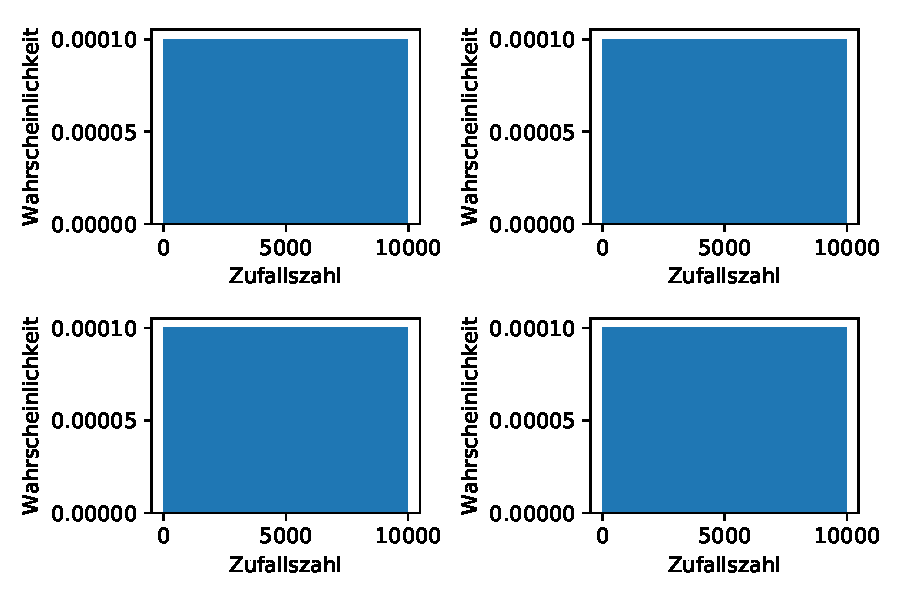
\includegraphics{Wahrschkeit.pdf}
  \caption{Wahrscheinlichkeit der erzeugten Zahle für verschiedene $x_.0$}
  \label{fig:Wahrkeit}
\end{figure}
\subsection*{c)}
In den Zeilen $177$-$201$ werden die zufällig generierten Werte $x_.n$ gegen $x_.{n+1}$ in einem 2D-Scatter-Plot und gegen $x_.{n+1}$ und $x_.{n+2}$ in einem 3D-Scatter-Plot aufgetragen. Wie in den Abbildungen \ref{fig:2D} und \ref{fig:3D} zu sehen ist, lassen sich auch hier deutliche Hyperebenen erkennen.
\begin{figure}
  \includegraphics{build/2D-Scatter-Plot.pdf}
  \caption{Paare aufeinanderfolgender Zahlen (selbst programmiert)}
  \label{fig:2D}
\end{figure}
\begin{figure}
  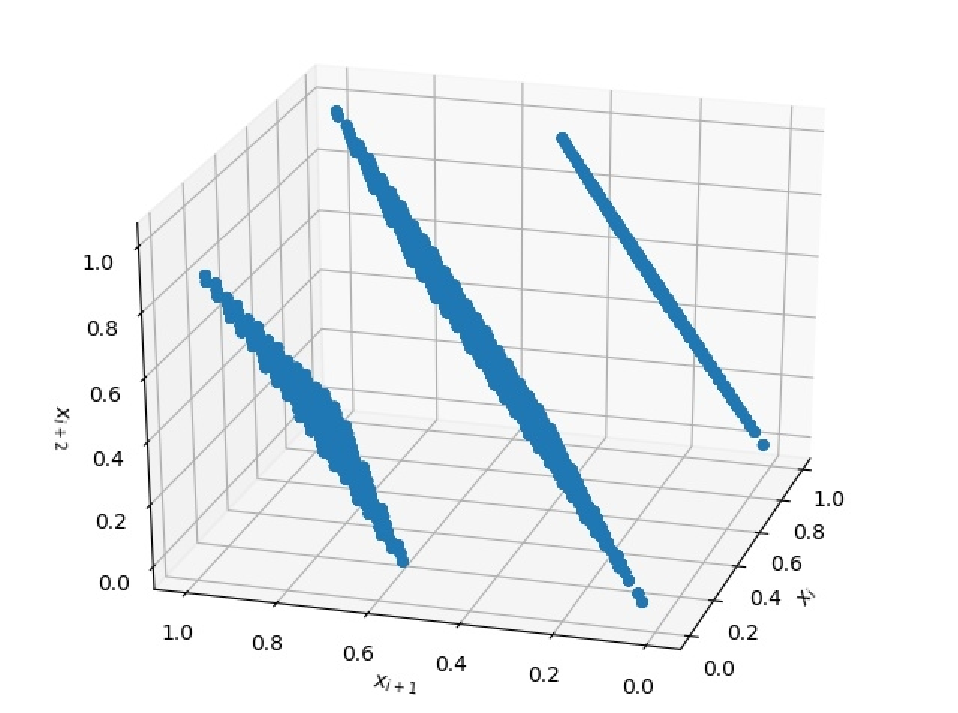
\includegraphics{3D-Scatter-Plot-gedreht.pdf}
  \caption{Tripletts aufeinanderfolgender Zahlen (selbst programmiert)}
  \label{fig:3D}
\end{figure}
\subsection*{d)}
Die Aufgabenteile $b)$ und $c)$ werden unter Verwendung von np.random.uniform() wiederholt. In den Abbildungen \ref{fig:Wahrkeit_rnd}bis \ref{fig:3D_rnd} ist zu erkennen, dass dieser Generator im Vergleich zum selbstgeschriebenen LKG wesentlich "zufälligere" Werte generiert.
\begin{figure}
  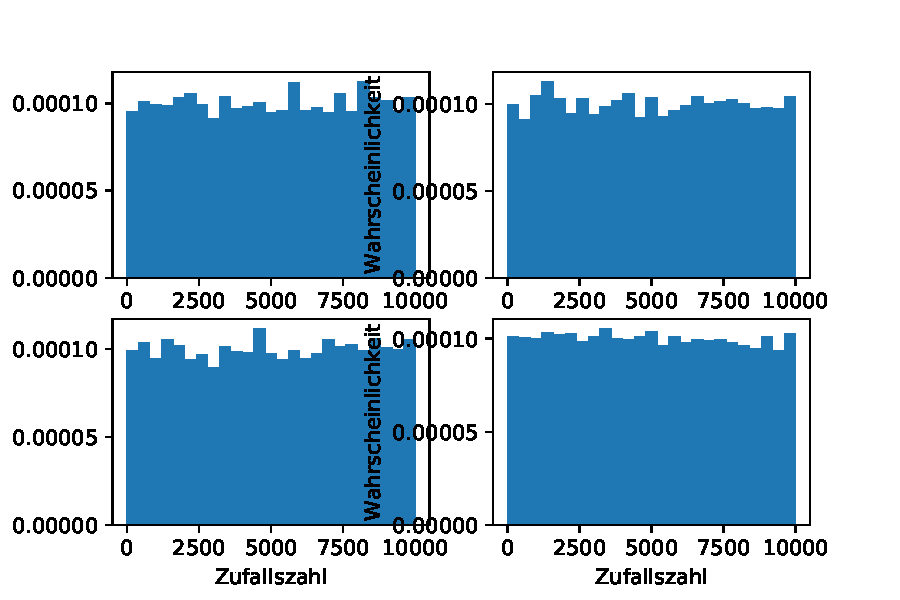
\includegraphics{Wahrschkeit_uniform.pdf}
  \caption{Wahrscheinlichkeit der erzeugten Zahlen für verschiedene $x_.0$}
  \label{fig:Wahrkeit_rnd}
\end{figure}
\begin{figure}
  \includegraphics{build/2D-Scatter-Plot-Uniform.pdf}
  \caption{Paare aufeinanderfolgender Zahlen (numpy.random.uniform())}
  \label{fig:2D_rnd}
\end{figure}
\begin{figure}
  \includegraphics{build/3D-Scatter-Plot-Uniform.pdf}
  \caption{Tripletts aufeinanderfolgender Zahlen (numpy.random.uniform())}
  \label{fig:3D_rnd}
\end{figure}
\subsection*{e)}
Es wird überprüft, mit welchem $x_.0$ der Generator aus Aufgabenteil $a)$
den Wert $\frac{1}{2}$ liefert. Für ganzzahlige Werte tritt dies sinnvoller Weise nie auf. Für Dezimalzahlen als Startwert wurde empirisch bestimmt, das für $x_.0 = 0,1 + 0,2n$, sowie für $x_.0 = 0,02n + 0,2k$ der Wert ein Mal pro Periode auftritt.
